\section{Hardware und Software}
Unsere, im zweiten Kapitel erwähnte, Mehrbenutzerleinwand bietet bis zu sechs Nutzern eine positionsabhängige, stereoskopische Perspektive auf eine virtuelle Szene. Sie wird von zwei Beamern betrieben, die mit einer Taktrate von jeweils 360 Hz in der Lage sind, jedem der insgesamt zwölf Shuttergläsern eine Frequenz von 60 Hz zu liefern. Somit nehmen die Nutzer die gemeinsame Umgebung gleichzeitig und unverzerrt aus ihrer jeweiligen getrackten Perspektive wahr. Die Dimensionen der Leinwand messen 4,20 Meter Weite und 2,60 Meter Länge bei einer Auflösung von 1920x1200 Pixeln.

\begin{figure}[h]
  \centering
  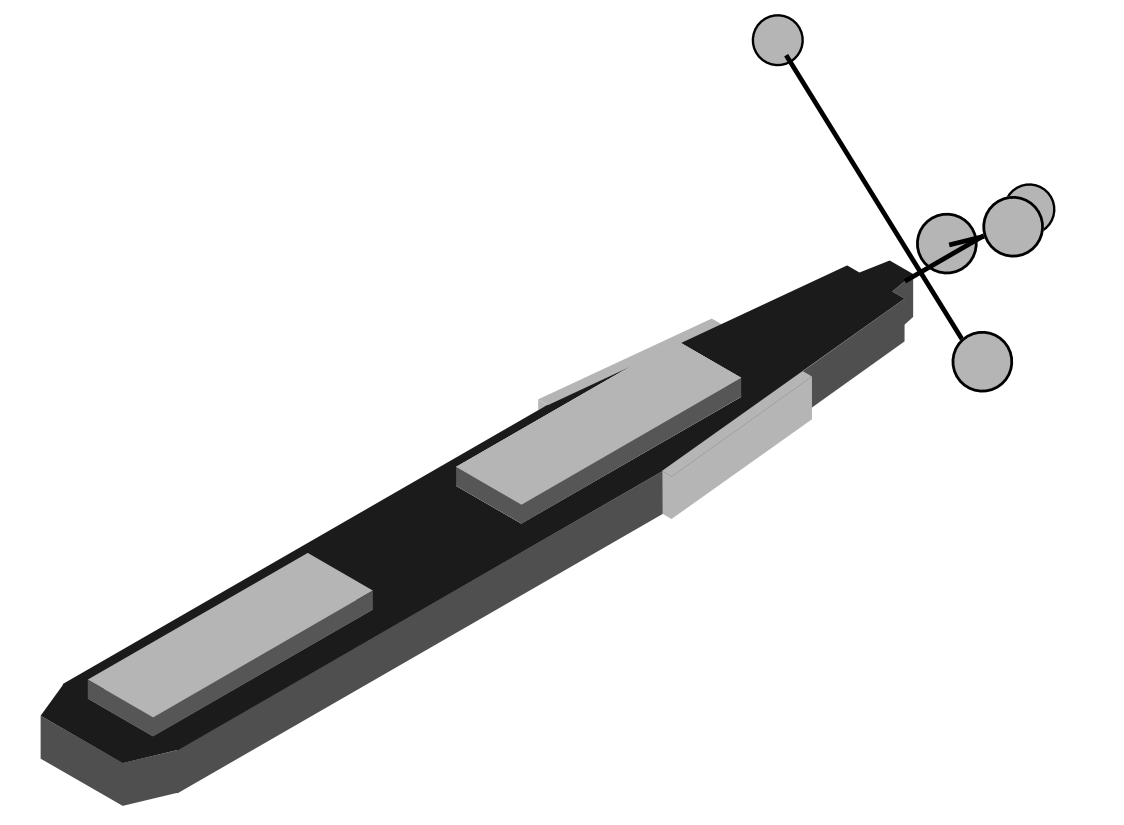
\includegraphics[width=0.5\textwidth]{images/pointer.png}
  \caption{Der getrackte Pointer wird als Eingabegerät genutzt.}
  \label{fig:todo}
\end{figure}

Als Eingabegeräte dienen sogenannte \glqq Pointer \grqq{}, deren Position und Ausrichtung im Raum ebenfalls vom System getrackt wird.

Die gesamte Implementierung wird im VR Framework Avango-Guacamole \cite{Schneegans2014Guacamole-AnShading} vorgenommen.

\section{Umgebung}



\begin{figure}[h]
  \centering
  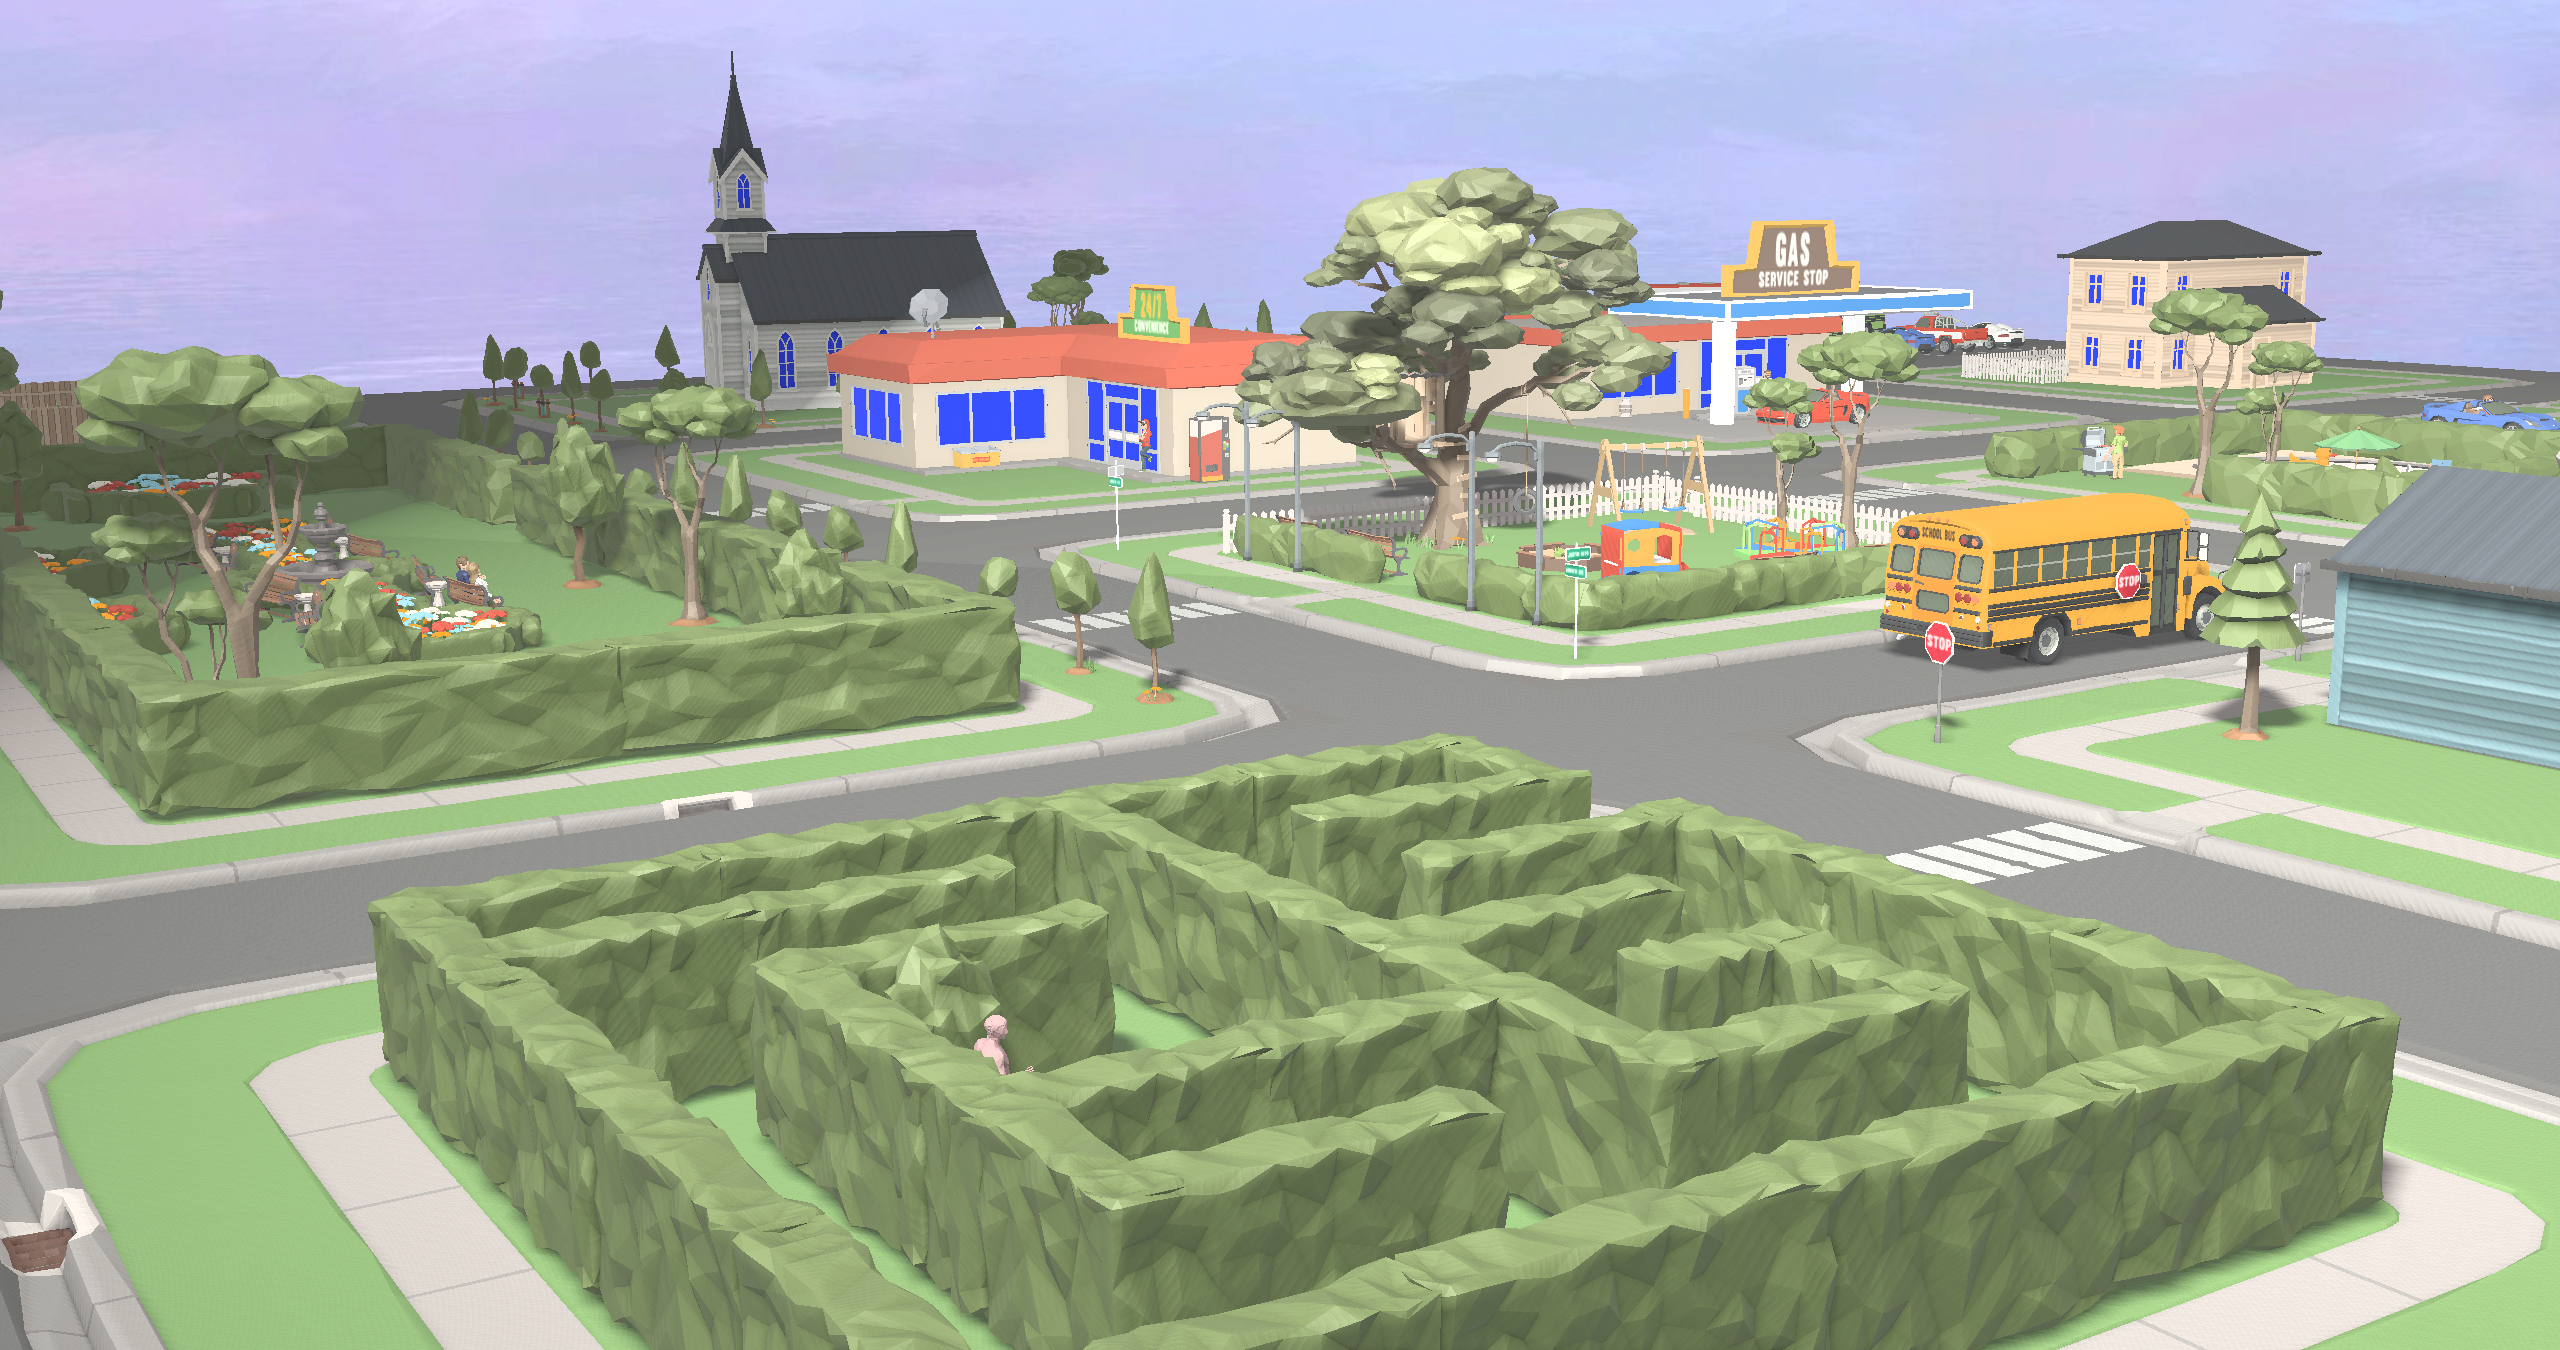
\includegraphics[width=\textwidth]{images/map2.png}
  \caption{Der Blick über die Testumgebung Richtung Nord-Osten.}
  \label{fig:todo}
\end{figure}

Um eine geeignete Testumgebung zu erhalten wurde im Rahmen einer HiWi-Stelle eine Nachbarschaft gebaut, welche sich dadurch auszeichnet, dass sie aus einzelnen \glqq Inseln \grqq{} besteht, welche einfach umgestellt werden können. Das genutzte Asset-Pack\footnote{https://www.cgtrader.com/3d-models/exterior/house/polygon-town-pack} kommt mit der Nutzung von sehr wenigen Polygonen aus, was die Rechenleistung bei der Bildberechnung auf der Grafikkarte minimiert und somit für schnellere Hertzraten sorgt.

\begin{figure}[h]
  \centering
  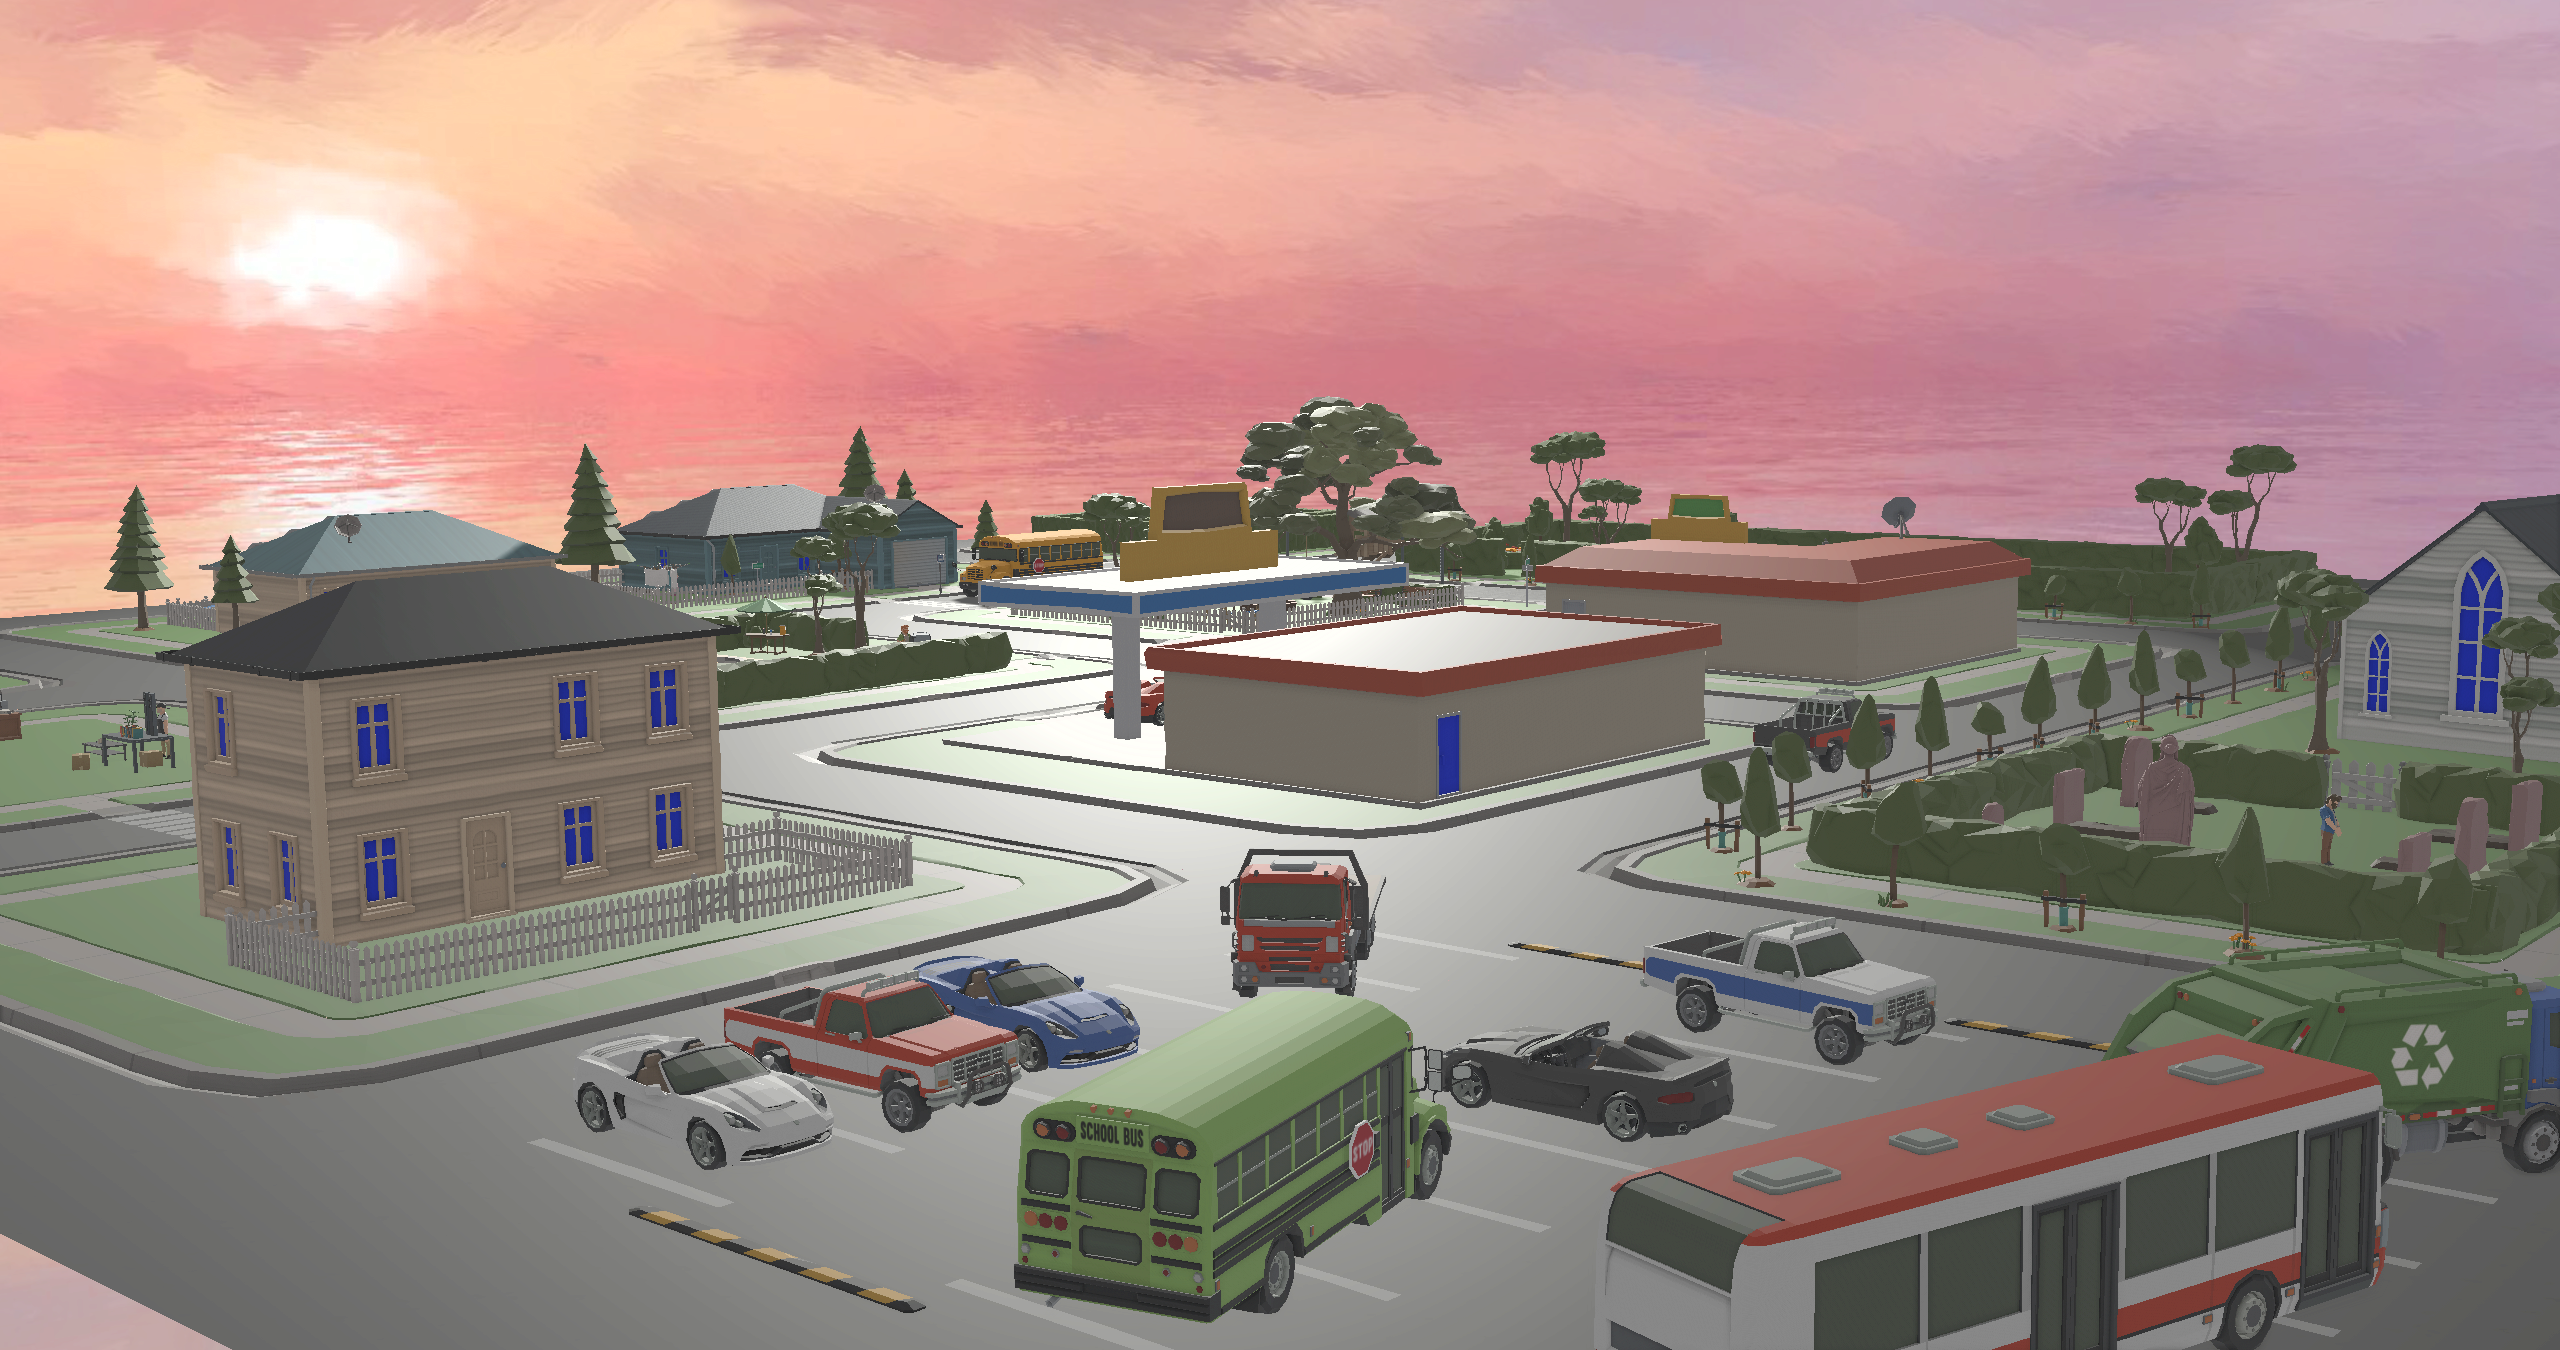
\includegraphics[width=\textwidth]{images/map1.png}
  \caption{Auch, wenn die untergehende Sonne etwas anderes vermuten lässt: Der Blick über die Testumgebung Richtung Süd-Westen.}
  \label{fig:todo}
\end{figure}
